\documentclass[11pt,a4paper]{article}

%% ── Core packages ────────────────────────────────────────────────────────────
\usepackage[a4paper, top=18mm, bottom=18mm, left=18mm, right=18mm]{geometry}
\usepackage[table]{xcolor}
\usepackage{amsmath,amssymb}
\usepackage{booktabs}
\usepackage{colortbl}
\usepackage{tabularx}
\usepackage{array}
\usepackage{multirow}
\usepackage{graphicx}
\usepackage{microtype}
\usepackage{parskip}
\usepackage{enumitem}
\usepackage{fontawesome5}
\usepackage{helvet}
\usepackage{mdframed}
\usepackage{fancyhdr}
\usepackage{lastpage}
\usepackage{eso-pic}
\usepackage{tikz}
\usepackage[most]{tcolorbox}

\usetikzlibrary{positioning,calc,shapes.geometric,backgrounds,patterns,decorations.pathmorphing}

\renewcommand{\familydefault}{\sfdefault}

%% ── Colour palette ───────────────────────────────────────────────────────────
\definecolor{PathBlue}{HTML}{1A3A5C}
\definecolor{PathTeal}{HTML}{2A7F7F}
\definecolor{PathGold}{HTML}{C8922A}
\definecolor{PathCream}{HTML}{F7F4EF}
\definecolor{PathLightBlue}{HTML}{E8F0F7}
\definecolor{PathLightTeal}{HTML}{E0F0F0}
\definecolor{PathMidGray}{HTML}{6B7280}
\definecolor{PathLightGray}{HTML}{F0F0F0}
\definecolor{PathRed}{HTML}{B8374A}
\definecolor{PathGreen}{HTML}{2E7D5E}
\definecolor{WatermarkGray}{HTML}{CCCCCC}

%% ── SPECIMEN watermark ───────────────────────────────────────────────────────
\AddToShipoutPictureBG{%
  \begin{tikzpicture}[remember picture, overlay]
    \node[
      rotate=45,
      opacity=0.07,
      font=\fontsize{88}{88}\selectfont\bfseries,
      text=PathMidGray
    ] at (current page.center) {SPECIMEN};
  \end{tikzpicture}%
}

%% ── Page style ───────────────────────────────────────────────────────────────
\pagestyle{fancy}
\fancyhf{}
\renewcommand{\headrulewidth}{0pt}
\fancyfoot[L]{\footnotesize\color{PathMidGray} Meridian Pathology Institute \textbullet{} Confidential Medical Record}
\fancyfoot[C]{\footnotesize\color{PathMidGray} Path.\,\#\ MPI-2024-0847}
\fancyfoot[R]{\footnotesize\color{PathMidGray} Page \thepage\ of \pageref{LastPage}}

%% ── tcolorbox styles ─────────────────────────────────────────────────────────
\tcbset{
  pathbase/.style={
    enhanced, arc=3pt, boxrule=0.6pt,
    left=6pt, right=6pt, top=5pt, bottom=5pt
  },
  sectionbox/.style={
    pathbase,
    colframe=PathBlue, colback=PathLightBlue,
    fonttitle=\bfseries\small\color{white},
    coltitle=white, attach boxed title to top left={yshift=-2mm,xshift=4mm},
    boxed title style={colback=PathBlue, arc=2pt, boxrule=0pt, left=4pt, right=4pt}
  },
  tealbox/.style={
    pathbase,
    colframe=PathTeal, colback=PathLightTeal,
    fonttitle=\bfseries\small\color{white},
    coltitle=white, attach boxed title to top left={yshift=-2mm,xshift=4mm},
    boxed title style={colback=PathTeal, arc=2pt, boxrule=0pt, left=4pt, right=4pt}
  },
  goldbox/.style={
    pathbase,
    colframe=PathGold, colback=PathCream,
    fonttitle=\bfseries\small\color{white},
    coltitle=white, attach boxed title to top left={yshift=-2mm,xshift=4mm},
    boxed title style={colback=PathGold, arc=2pt, boxrule=0pt, left=4pt, right=4pt}
  },
  diagnosisbox/.style={
    pathbase,
    colframe=PathBlue, colback=PathBlue,
    fonttitle=\bfseries\normalsize\color{white},
    coltitle=white
  },
  critbox/.style={
    pathbase,
    colframe=PathRed, colback=PathRed!8,
    fonttitle=\bfseries\small\color{white},
    coltitle=white, attach boxed title to top left={yshift=-2mm,xshift=4mm},
    boxed title style={colback=PathRed, arc=2pt, boxrule=0pt, left=4pt, right=4pt}
  },
  infostrip/.style={
    pathbase, colframe=PathLightGray, colback=PathLightGray,
    boxrule=0pt, arc=2pt
  }
}

%% ── Helpers ──────────────────────────────────────────────────────────────────
\newcommand{\fieldlabel}[1]{\textcolor{PathMidGray}{\footnotesize\textbf{#1}}}
\newcommand{\fieldval}[1]{\textcolor{PathBlue}{\small #1}}
\newcommand{\posmarker}{\textcolor{PathGreen}{\faCheckCircle}}
\newcommand{\negmarker}{\textcolor{PathMidGray}{\faTimesCircle}}
\newcommand{\critmarker}{\textcolor{PathRed}{\faExclamationCircle}}

\newcolumntype{L}[1]{>{\raggedright\arraybackslash}p{#1}}
\newcolumntype{C}[1]{>{\centering\arraybackslash}p{#1}}
\newcolumntype{R}[1]{>{\raggedleft\arraybackslash}p{#1}}

\setlength{\parindent}{0pt}
\setlength{\parskip}{4pt}

%% ═══════════════════════════════════════════════════════════════════════════════
\begin{document}

%% ── HEADER ───────────────────────────────────────────────────────────────────
\begin{tikzpicture}[remember picture, overlay]
  \fill[PathBlue] (current page.north west) rectangle +(\paperwidth, -28mm);
  \fill[PathTeal] (current page.north west) ++(0,-28mm) rectangle +(\paperwidth, -3mm);
  \fill[PathGold] (current page.north west) ++(0,-31mm) rectangle +(\paperwidth, -1.5mm);
\end{tikzpicture}

\vspace*{-6pt}
\begin{minipage}[t]{0.62\textwidth}
  \vspace{0pt}
  {\color{white}\fontsize{22}{26}\selectfont\bfseries Pathology \& Histology}\\[2pt]
  {\color{PathGold}\fontsize{13}{16}\selectfont\bfseries Analysis Report}\\[4pt]
  {\color{white!80!PathBlue}\footnotesize Meridian Pathology Institute \textbullet{} Department of Anatomical Pathology}
\end{minipage}%
\begin{minipage}[t]{0.38\textwidth}
  \vspace{0pt}
  \raggedleft
  \begin{tikzpicture}
    \node[draw=white, line width=1.2pt, rounded corners=4pt,
          fill=white!15!PathBlue, text=white,
          inner xsep=8pt, inner ysep=6pt, align=center] {%
      {\bfseries\large MPI-2024-0847}\\[2pt]
      {\footnotesize\faCalendar\quad Reported: 14 November 2024}\\[1pt]
      {\footnotesize\faClock\quad Received: 11 November 2024}\\[1pt]
      {\footnotesize\faFlask\quad Biopsy \textbullet{} Surgical Specimen}
    };
  \end{tikzpicture}
\end{minipage}

\vspace{20mm}

%% ── PATIENT & CLINICAL INFO ──────────────────────────────────────────────────
\begin{tcolorbox}[sectionbox, title={\faUser\quad Patient \& Clinical Information}]
\begin{minipage}[t]{0.48\linewidth}
  \vspace{0pt}
  \fieldlabel{Patient Name}\\
  \fieldval{\textbf{Margaret L. Harrington}}\\[6pt]
  \fieldlabel{Date of Birth}\\
  \fieldval{03 April 1962 \quad (Age: 62)}\\[6pt]
  \fieldlabel{Patient ID}\\
  \fieldval{PT-\#{}H-883421}\\[6pt]
  \fieldlabel{Gender}\\
  \fieldval{Female}\\[6pt]
  \fieldlabel{Referring Physician}\\
  \fieldval{Dr.\ Thomas A. Wentworth, MD}\\[6pt]
  \fieldlabel{Institution}\\
  \fieldval{Synapse General Hospital, Ward 7-B}
\end{minipage}%
\begin{minipage}[t]{0.04\linewidth}
  \vspace{0pt}
\end{minipage}%
\begin{minipage}[t]{0.48\linewidth}
  \vspace{0pt}
  \fieldlabel{Clinical Indication}\\
  \fieldval{Right breast mass, suspicious on imaging; BI-RADS 4C}\\[6pt]
  \fieldlabel{Specimen Type}\\
  \fieldval{Core needle biopsy \texttimes{} 4 cores, right breast (2:00 position)}\\[6pt]
  \fieldlabel{Gross Description}\\
  \fieldval{Four tan-white cylindrical cores, each approx.\ 12\,mm in length and 1.5\,mm in diameter, submitted in entirety in one block.}\\[6pt]
  \fieldlabel{Clinical History}\\
  \fieldval{Palpable lump noted 6 weeks prior; no prior breast biopsies; family history of breast carcinoma (maternal aunt).}
\end{minipage}
\end{tcolorbox}

\vspace{4pt}

%% ── GROSS EXAMINATION & PROCESSING ──────────────────────────────────────────
\begin{minipage}[t]{0.485\linewidth}
\begin{tcolorbox}[tealbox, title={\faSearch\quad Gross Examination}]
  \setlength{\parskip}{3pt}
  \fieldlabel{Specimen Condition}\\
  \fieldval{Received fresh, immediately fixed in 10\% neutral buffered formalin}\\[5pt]
  \fieldlabel{Dimensions}\\
  \fieldval{Aggregate tissue: 4.8\,cm \texttimes{} 0.15\,cm}\\[5pt]
  \fieldlabel{Colour / Texture}\\
  \fieldval{Tan-white, firm; no haemorrhage or necrosis on gross inspection}\\[5pt]
  \fieldlabel{Cassettes Submitted}\\
  \fieldval{1 cassette (A1) -- all cores in toto}\\[5pt]
  \fieldlabel{Fixation Time}\\
  \fieldval{6--8 hours (ASCO/CAP compliant)}
\end{tcolorbox}
\end{minipage}%
\hfill
\begin{minipage}[t]{0.485\linewidth}
\begin{tcolorbox}[tealbox, title={\faCog\quad Processing \& Staining}]
  \setlength{\parskip}{3pt}
  \fieldlabel{Tissue Processing}\\
  \fieldval{Standard overnight automated processor; paraffin embedded}\\[5pt]
  \fieldlabel{Sectioning}\\
  \fieldval{5\,\textmu{}m sections, 3 levels}\\[5pt]
  \fieldlabel{Routine Stain}\\
  \fieldval{Haematoxylin \& Eosin (H\&{}E)}\\[5pt]
  \fieldlabel{Special Stains}\\
  \fieldval{Periodic Acid--Schiff (PAS); Masson Trichrome}\\[5pt]
  \fieldlabel{Immunohistochemistry Panel}\\
  \fieldval{ER, PR, HER2, Ki-67, CK5/6, p63, CD44}
\end{tcolorbox}
\end{minipage}

\par\vspace{4pt}

%% ── MICROSCOPIC FINDINGS ─────────────────────────────────────────────────────
\begin{tcolorbox}[sectionbox, title={\faMicroscope\quad Microscopic Findings}]

\textbf{\color{PathBlue}Architectural Pattern}\\[2pt]
The cores show infiltration by a malignant epithelial proliferation arranged predominantly in
irregular solid nests and single-file cords (\emph{Indian-file pattern}) traversing a desmoplastic
stroma. Focal gland formation is present, accounting for approximately 10--15\% of the tumour
volume. No evidence of lobular in situ carcinoma is identified in the adjacent tissue.

\vspace{6pt}
\textbf{\color{PathBlue}Cytological Features}

\begin{itemize}[leftmargin=1.6em, itemsep=2pt, topsep=2pt]
  \item Tumour cells are large with moderate-to-abundant eosinophilic cytoplasm and
        markedly pleomorphic nuclei (nuclear grade 3).
  \item Nuclear:cytoplasmic ratio is high; prominent macronucleoli present in the majority
        of cells.
  \item Mitotic figures: 12 per 10 high-power fields (HPF), including atypical forms.
  \item Intracytoplasmic lumina (ICL) focally present; mucin-positive on PAS stain.
\end{itemize}

\vspace{6pt}
\textbf{\color{PathBlue}Stromal Characteristics}\\[2pt]
Moderate desmoplastic stroma; scattered lymphocytic infiltrate (TIL score $\approx$ 15\%).
Masson Trichrome highlights an increase in collagen deposition around tumour nests.
No vascular or lymphatic invasion identified on H\&{}E or D2-40 staining.

\vspace{6pt}
\textbf{\color{PathBlue}Associated Findings}\\[2pt]
Adjacent non-neoplastic breast tissue demonstrates columnar cell change with atypia (flat
epithelial atypia, FEA). Microcalcifications are present in association with both the
tumour nests and the benign lobules.

\end{tcolorbox}

\vspace{4pt}

%% ── IHC RESULTS TABLE ────────────────────────────────────────────────────────
\begin{tcolorbox}[goldbox, title={\faTable\quad Immunohistochemistry Results}]

\renewcommand{\arraystretch}{1.35}
\begin{tabularx}{\linewidth}{L{2.6cm} C{1.8cm} C{2.2cm} C{1.6cm} X}
  \toprule
  \rowcolor{PathGold!20}
  \textbf{Marker} & \textbf{Result} & \textbf{Score / Extent} & \textbf{Clone} & \textbf{Interpretation} \\
  \midrule
  ER (Oestrogen R.) & \posmarker\ \textbf{Positive} & Allred 7/8 (90\%{}, 3+) & SP1 & Strong nuclear positivity \\
  \rowcolor{PathLightGray!60}
  PR (Progesterone R.) & \posmarker\ \textbf{Positive} & Allred 6/8 (60\%{}, 3+) & 1E2 & Moderate nuclear positivity \\
  HER2 (c-erbB2) & \negmarker\ Negative & Score 1+ & 4B5 & Incomplete faint membrane staining \\
  \rowcolor{PathLightGray!60}
  Ki-67 (MIB-1) & \critmarker\ Elevated & 28\%{} of nuclei & 30-9 & High proliferative index \\
  CK5/6 & \negmarker\ Negative & 0\%{} & D5/16B4 & No basal phenotype \\
  \rowcolor{PathLightGray!60}
  p63 & \negmarker\ Negative & 0\%{} & 4A4 & No myoepithelial layer \\
  CD44 & \posmarker\ Positive & 40\%{} (2+) & IM7 & Focal expression \\
  \bottomrule
\end{tabularx}

\vspace{4pt}
{\footnotesize\color{PathMidGray}%
\textbf{Note:} HER2 FISH reflex testing recommended per ASCO/CAP 2023 guidelines (Score 1+ borderline).
All controls performed satisfactorily. Automated staining platform: Meridian Benchmark ULTRA.}
\end{tcolorbox}

\newpage

%% ── GRADING TABLE ────────────────────────────────────────────────────────────
\begin{tcolorbox}[sectionbox, title={\faStar\quad Histological Grading --- Nottingham (Elston--Ellis)}]

\renewcommand{\arraystretch}{1.4}
\begin{tabularx}{\linewidth}{L{4.5cm} C{2.5cm} C{2.5cm} X}
  \toprule
  \rowcolor{PathBlue!12}
  \textbf{Parameter} & \textbf{Score} & \textbf{Maximum} & \textbf{Comment} \\
  \midrule
  Tubule Formation & 3 & 3 & \textless{}10\%{} tubule formation \\
  \rowcolor{PathLightBlue}
  Nuclear Pleomorphism & 3 & 3 & Marked vesicular nuclei with prominent nucleoli \\
  Mitotic Count & 3 & 3 & 12 mitoses / 10 HPF (field diameter 0.44\,mm) \\
  \midrule
  \rowcolor{PathGold!20}
  \textbf{Total Score} & \textbf{9/9} & \textbf{9} & \textbf{Grade 3 (Poorly Differentiated)} \\
  \bottomrule
\end{tabularx}

\vspace{4pt}
{\footnotesize\color{PathMidGray} Grading performed on H\&{}E-stained sections at 400\texttimes{} magnification
(Olympus BX53 with calibrated eyepiece reticule).}
\end{tcolorbox}

\vspace{4pt}

%% ── SPECIAL STAINS SUMMARY ───────────────────────────────────────────────────
\begin{minipage}[t]{0.485\linewidth}
\begin{tcolorbox}[tealbox, title={\faFlask\quad Special Stain Summary}]
\renewcommand{\arraystretch}{1.3}
\begin{tabular}{L{3.2cm} l}
  \toprule
  \rowcolor{PathLightTeal}
  \textbf{Stain} & \textbf{Findings} \\
  \midrule
  PAS (Periodic Acid--Schiff) & Focal positivity in ICL \\
  \rowcolor{PathLightGray!50}
  Masson Trichrome & Desmoplastic stroma \posmarker \\
  Alcian Blue (pH 2.5) & Focal mucin pools \\
  \rowcolor{PathLightGray!50}
  Reticulin & Disrupted framework \\
  \bottomrule
\end{tabular}
\end{tcolorbox}
\end{minipage}%
\hfill
\begin{minipage}[t]{0.485\linewidth}
\begin{tcolorbox}[tealbox, title={\faRuler\quad Measurements \& Quantitative Data}]
\renewcommand{\arraystretch}{1.3}
\begin{tabular}{L{4.0cm} l}
  \toprule
  \rowcolor{PathLightTeal}
  \textbf{Parameter} & \textbf{Value} \\
  \midrule
  Tumour extent (cores) & 3 of 4 cores positive \\
  \rowcolor{PathLightGray!50}
  Max.\ linear extent & 9.2\,mm \\
  Percentage core involved & 65\%{} \\
  \rowcolor{PathLightGray!50}
  TIL Score & $\approx$ 15\%{} \\
  Microcalcifications & Present \\
  \bottomrule
\end{tabular}
\end{tcolorbox}
\end{minipage}

\par\vspace{4pt}

%% ── DIFFERENTIAL DIAGNOSIS ───────────────────────────────────────────────────
\begin{tcolorbox}[goldbox, title={\faList\quad Differential Diagnosis Considered}]
\begin{enumerate}[leftmargin=1.8em, itemsep=3pt, topsep=2pt, label=\lbrack\arabic*\rbrack]
  \item \textbf{Invasive Ductal Carcinoma NST, Grade 3} \textcolor{PathGreen}{\faCheckCircle\ \textbf{FAVOURED}} ---
        Supported by solid/cord growth pattern, nuclear grade 3, desmoplastic stroma,
        ER/PR positivity, and absence of myoepithelial cells (p63, CK5/6 negative).
  \item \textbf{Invasive Lobular Carcinoma} \textcolor{PathMidGray}{--- Excluded} ---
        Indian-file pattern was initially considered; however, E-cadherin staining (performed
        reflexly) shows preserved membranous positivity, excluding lobular phenotype.
  \item \textbf{Metaplastic Carcinoma} \textcolor{PathMidGray}{--- Excluded} ---
        No squamous or mesenchymal differentiation identified; CK5/6 and p63 negative.
  \item \textbf{Phyllodes Tumour (malignant)} \textcolor{PathMidGray}{--- Excluded} ---
        No biphasic architecture; stromal overgrowth absent; epithelial nature confirmed by IHC.
\end{enumerate}
\end{tcolorbox}

\vspace{4pt}

%% ── MOLECULAR SUBTYPE BOX ────────────────────────────────────────────────────
\begin{minipage}[t]{0.485\linewidth}
\begin{tcolorbox}[sectionbox, title={\faDna\quad Surrogate Molecular Subtype}]
  \setlength{\parskip}{5pt}
  Based on IHC profile (St.\ Gallen 2023 consensus):

  \vspace{4pt}
  \begin{center}
  
\begin{tikzpicture}
    \node[draw=PathBlue, line width=1.5pt, fill=PathBlue,
          rounded corners=4pt, text=white,
          inner xsep=14pt, inner ysep=8pt, font=\bfseries\large] {%
      Luminal B (HER2-negative)};
  \end{tikzpicture}
  \end{center}

  \vspace{4pt}
  {\small
  \begin{tabular}{@{}ll@{}}
    ER: & Positive ($\geq 1\%$) \\
    PR: & Positive ($\geq 20\%$) \\
    HER2: & Negative \\
    Ki-67: & High ($\geq 20\%$) \\
  \end{tabular}}

  \vspace{4pt}
  {\footnotesize\color{PathMidGray}
  Oncotype DX / Prosigna testing may be considered per MDT guidelines.}
\end{tcolorbox}
\end{minipage}%
\hfill
\begin{minipage}[t]{0.485\linewidth}
\begin{tcolorbox}[critbox, title={\faExclamationTriangle\quad Critical / Actionable Findings}]
  \setlength{\parskip}{5pt}
  \begin{itemize}[leftmargin=1.4em, itemsep=3pt, topsep=2pt]
    \item[\critmarker] \textbf{Malignancy confirmed} --- Immediate MDT referral required.
    \item[\critmarker] \textbf{Ki-67 28\%{}} --- Indicates high proliferative activity; discuss
          adjuvant chemotherapy with oncology team.
    \item[\critmarker] \textbf{HER2 Score 1+} --- FISH reflex testing ordered (specimen block A1
          forwarded to Vertex Molecular Diagnostics Laboratory).
    \item[\critmarker] \textbf{FEA in adjacent tissue} --- Bilateral surveillance imaging recommended.
  \end{itemize}
  \vspace{2pt}
  {\footnotesize\color{PathRed!80!black}%
  Referring clinician notified by telephone: 14 Nov 2024, 09:47 hrs.}
\end{tcolorbox}
\end{minipage}

\par\vspace{4pt}

%% ── FINAL DIAGNOSIS ──────────────────────────────────────────────────────────
\begin{tcolorbox}[diagnosisbox, title={}]
  \begin{center}
  {\color{PathGold}\bfseries\large FINAL DIAGNOSIS}\\[4pt]
  \end{center}
  \color{white}
  \textbf{Site:} Right breast, 2:00 position --- core needle biopsy\\[4pt]
  \textbf{Diagnosis:}\\[2pt]
  \quad INVASIVE BREAST CARCINOMA OF NO SPECIAL TYPE (NST)\\
  \quad Nottingham Grade 3 (Score 9/9)\\
  \quad ER: Positive (Allred 7/8) \textbar{} PR: Positive (Allred 6/8) \textbar{} HER2: 1+ (FISH pending) \textbar{} Ki-67: 28\%\\[4pt]
  \textbf{Associated Findings:}\\[2pt]
  \quad Flat Epithelial Atypia (FEA) in adjacent non-neoplastic breast tissue\\
  \quad Microcalcifications present\\[4pt]
  \textbf{Staging Correlate (pathological biopsy):}\\[2pt]
  \quad pTx (size not assessable on core biopsy) N0 M0 per AJCC 8th Ed.\\
  \quad Final staging to be assigned post-excision.
\end{tcolorbox}

\newpage

%% ── MICROSCOPIC DIAGRAM ──────────────────────────────────────────────────────
\begin{tcolorbox}[sectionbox, title={\faImage\quad Schematic Representation of Microscopic Architecture}]
\begin{center}
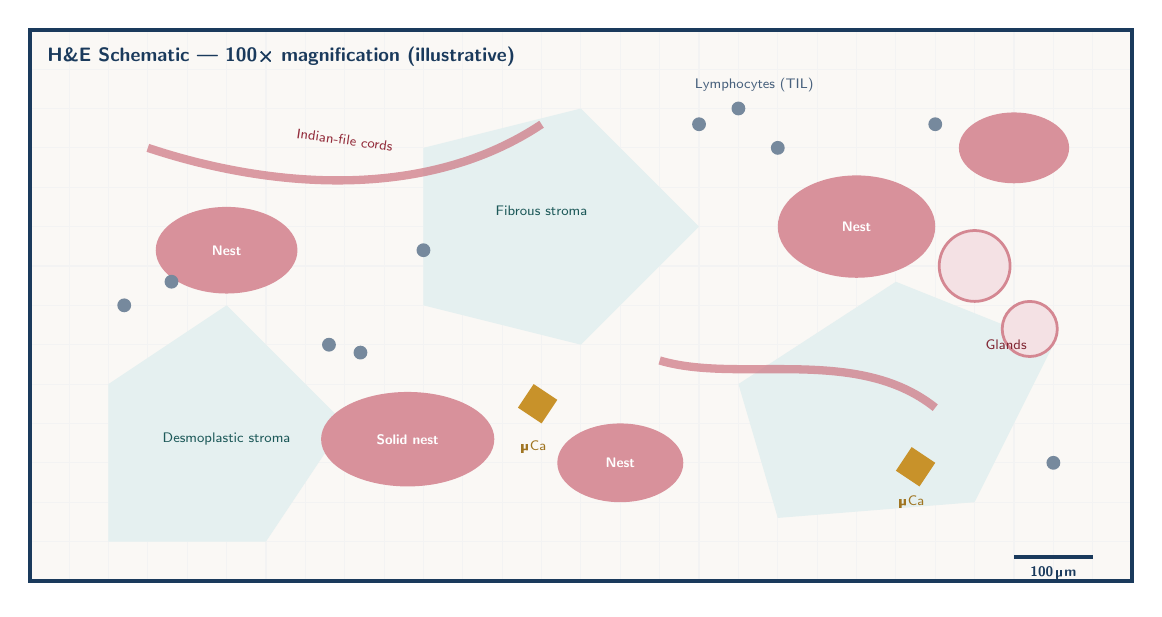
\begin{tikzpicture}[scale=1.0]
  %% Background tissue
  \fill[PathCream!60] (0,0) rectangle (14,7);
  \draw[PathLightGray!80, line width=0.4pt, step=0.5] (0,0) grid (14,7);

  %% Desmoplastic stroma regions
  \fill[PathTeal!12] (1,0.5) -- (3,0.5) -- (4,2) -- (2.5,3.5) -- (1,2.5) -- cycle;
  \fill[PathTeal!12] (5,3.5) -- (7,3) -- (8.5,4.5) -- (7,6) -- (5,5.5) -- cycle;
  \fill[PathTeal!12] (9.5,0.8) -- (12,1) -- (13,3) -- (11,3.8) -- (9,2.5) -- cycle;
  \node[font=\tiny, color=PathTeal!70!black] at (2.5,1.8) {Desmoplastic stroma};
  \node[font=\tiny, color=PathTeal!70!black] at (6.5,4.7) {Fibrous stroma};

  %% Tumour nests (solid)
  \fill[PathRed!55] (2.5,4.2) ellipse ({0.9} and {0.55});
  \fill[PathRed!55] (4.8,1.8) ellipse ({1.1} and {0.6});
  \fill[PathRed!55] (7.5,1.5) ellipse ({0.8} and {0.5});
  \fill[PathRed!55] (10.5,4.5) ellipse ({1.0} and {0.65});
  \fill[PathRed!55] (12.5,5.5) ellipse ({0.7} and {0.45});
  \node[font=\tiny\bfseries, color=white] at (2.5,4.2) {Nest};
  \node[font=\tiny\bfseries, color=white] at (4.8,1.8) {Solid nest};
  \node[font=\tiny\bfseries, color=white] at (7.5,1.5) {Nest};
  \node[font=\tiny\bfseries, color=white] at (10.5,4.5) {Nest};

  %% Indian file cords
  \draw[PathRed!70, line width=3pt, opacity=0.7]
    (1.5,5.5) .. controls (3,5) and (5,4.8) .. (6.5,5.8);
  \draw[PathRed!70, line width=3pt, opacity=0.7]
    (8,2.8) .. controls (9,2.5) and (10.5,3) .. (11.5,2.2);
  \node[font=\tiny, color=PathRed!80!black, rotate=-8] at (4,5.6) {Indian-file cords};

  %% Lymphocyte infiltrate (small dots)
  \foreach \x/\y in {1.2/3.5, 1.8/3.8, 3.8/3.0, 4.2/2.9, 5.0/4.2,
                      8.5/5.8, 9.0/6.0, 9.5/5.5, 11.5/5.8, 13/1.5} {%
    \fill[PathBlue!60] (\x,\y) circle (2.5pt);
  }
  \node[font=\tiny, color=PathBlue!80] at (9.2,6.3) {Lymphocytes (TIL)};

  %% Microcalcification
  \fill[PathGold] (6.2,2.2) -- (6.5,2.0) -- (6.7,2.3) -- (6.4,2.5) -- cycle;
  \fill[PathGold] (11.0,1.4) -- (11.3,1.2) -- (11.5,1.5) -- (11.2,1.7) -- cycle;
  \node[font=\tiny, color=PathGold!80!black] at (6.4,1.7) {\textmu{}Ca};
  \node[font=\tiny, color=PathGold!80!black] at (11.2,1.0) {\textmu{}Ca};

  %% Gland formation
  \draw[PathRed!60, fill=PathRed!15, line width=1pt]
    (12,4.0) circle (0.45);
  \draw[PathRed!60, fill=PathRed!15, line width=1pt]
    (12.7,3.2) circle (0.35);
  \node[font=\tiny, color=PathRed!70!black] at (12.4,3.0) {Glands};

  %% Boundary box
  \draw[PathBlue, line width=1.5pt] (0,0) rectangle (14,7);

  %% Scale bar
  \draw[PathBlue, line width=1.5pt] (12.5,0.3) -- (13.5,0.3);
  \node[below, font=\tiny\bfseries, color=PathBlue] at (13,0.3) {100\,\textmu{}m};

  %% Legend
  \node[anchor=north west, font=\scriptsize\bfseries, color=PathBlue] at (0.1,6.9) {H\&{}E Schematic --- 100\texttimes{} magnification (illustrative)};
\end{tikzpicture}
\end{center}
\end{tcolorbox}

\vspace{4pt}

%% ── CLINICAL CORRELATIONS & RECOMMENDATIONS ──────────────────────────────────
\begin{tcolorbox}[goldbox, title={\faClipboardList\quad Clinical Correlations \& Pathologist Recommendations}]
  \setlength{\parskip}{4pt}

  \textbf{\color{PathBlue}1.\ Surgical Management}\\
  Surgical excision with sentinel lymph node biopsy is recommended. Wide local excision
  (breast-conserving surgery) vs.\ mastectomy to be determined by the MDT following
  MRI staging. Clip marker placed at biopsy site for surgical localisation.

  \textbf{\color{PathBlue}2.\ Systemic Therapy Consideration}\\
  Luminal B (HER2-negative) subtype with Ki-67 of 28\%{} and Grade 3 morphology warrants
  discussion of adjuvant chemotherapy in addition to standard endocrine therapy
  (aromatase inhibitor recommended given post-menopausal status).

  \textbf{\color{PathBlue}3.\ Genomic Testing}\\
  Oncotype DX Recurrence Score or Prosigna (PAM50) testing may refine chemotherapy
  decision-making in this pN0 setting (per NICE DG34 guidance).

  \textbf{\color{PathBlue}4.\ HER2 FISH Reflex}\\
  HER2 FISH has been requested reflexly. Results expected within 5 business days.
  Block A1 retained at Meridian Pathology Institute for FISH and future ancillary studies.

  \textbf{\color{PathBlue}5.\ Surveillance of Contralateral Breast}\\
  FEA identified in adjacent tissue and family history of breast carcinoma indicate
  annual bilateral MRI surveillance per Apex Breast Imaging Network protocol.
\end{tcolorbox}

\vspace{4pt}

%% ── QUALITY ASSURANCE ────────────────────────────────────────────────────────
\begin{minipage}[t]{0.485\linewidth}
\begin{tcolorbox}[infostrip]
  {\small\bfseries\color{PathBlue}\faLock\quad Quality Assurance}\\[4pt]
  {\footnotesize
  \begin{tabular}{@{}L{3.0cm} l@{}}
    Slide review: & Dr.\ Clara S. Okafor, MD \\
    Second opinion: & Dr.\ James Whitfield, FRCPath \\
    QA status: & \textcolor{PathGreen}{\faCheckCircle\ Passed} \\
    EQA scheme: & Nimbus Pathology EQA 2024 \\
    Turnaround: & 3 calendar days \\
  \end{tabular}}
\end{tcolorbox}
\end{minipage}%
\hfill
\begin{minipage}[t]{0.485\linewidth}
\begin{tcolorbox}[infostrip]
  {\small\bfseries\color{PathBlue}\faSignature\quad Pathologist Authorisation}\\[4pt]
  {\footnotesize
  \begin{tabular}{@{}L{3.0cm} l@{}}
    Reporting Pathologist: & Dr.\ Clara S. Okafor, MD\\
    Qualification: & MBBCh, FRCPath, PhD \\
    Date Authorised: & 14 November 2024 \\
    Digital Signature: & \texttt{[Digitally signed -- MPI]}\\
    Report Status: & \textcolor{PathGreen}{\textbf{FINAL}} \\
  \end{tabular}}
\end{tcolorbox}
\end{minipage}

\par\vspace{4pt}

%% ── FOOTER DISCLAIMER ────────────────────────────────────────────────────────
\begin{tcolorbox}[pathbase, colframe=PathMidGray!40, colback=PathLightGray, arc=2pt,
                  left=5pt, right=5pt, top=4pt, bottom=4pt]
{\footnotesize\color{PathMidGray}
\textbf{DISCLAIMER:} This report is intended solely for the use of the requesting clinician and is based on the specimen(s) submitted.
Pathological diagnosis must always be correlated with clinical, radiological, and other findings.
This report has been generated for specimen MPI-2024-0847 at Meridian Pathology Institute, 42 Helix Boulevard, Nexa Medical Quarter, NQ1 4PL.
\textbf{All patient and clinician details in this specimen are fictitious.}
Unauthorised disclosure of this document is prohibited under data protection legislation.
\hfill \faLock\ Encrypted Report}
\end{tcolorbox}

\end{document}
